
\chapter{Results}

In this chapter, different approaches for training the YOLO model are presented. First, the results of training a simple large model will show a baseline model which is then improved by different settings. Afterwards, the results of training the small and medium model are shown. Finally, the three different model sizes are compared.

\section{Large Network}

The first experiments were made with only a small part of the data set being manually labeled. At first, the images of the TUM data that contain approximately one big sugar beet per image were labeled automatically with \texttt{0 0.5 0.5 1 1}. This means that the whole picture is labeled as containing exactly one sugar beet. We assumed that these images were already in the perfect format for our use case and the automatic labeling would be sufficient. The images containing multiple small plants are labeled manually and exactly. The model was trained with default hyperparameters and settings. This means that the number of epochs is 300, box loss gain of 0.05, class loss gain of 0.5, object loss gain of 1.0 and IoU threshold for training of 0.2. The data augmentation values can be found in table \ref{tab:augmentation_exp1}.

\begin{table}[h!]
	\centering
	\begin{tabular}{|c c c c c c c c c c c|} 
		\hline
		Hue & Sat & Value & Degrees & Translate & Scale & Shear & Persp & UD & LR & Mosaic \\ % [0.5ex] 
		\hline
		0.015 & 0.7 & 0.4 & 0.0 & 0.1 & 0.5 & 0.0 & 0.0 & 0.0 & 0.5 & 1.0 \\
		\hline
	\end{tabular}
	\caption{Values for data augmentation}
	\label{tab:augmentation_exp1}
\end{table}

All in all, small data augmentation is used. $ 85\% $ of the data was used as training set and $ 15\% $ as validation set.\\

For the training and validation set, the results were accurate. With a real number of 9110 sugar beets and a detected number of plants of 8162, this results in an accuracy of $ 89,6\% $. Although for new, unseen images, the accuracy is very low. Here, the number of labeled sugar beets is 575 and only 68 are detected. An overall accuracy of $ 11,8\% $ results. In this experiment, only the number of detected and real sugar beets are observed, not the location or size of the bounding boxes. However, the results show that this model is not sufficient for detecting the boundaries of sugar beets. Two examples of detected objects can be seen in figure \ref{fig:results_experiment_1}.

\begin{figure}[htb!]
	\centering
	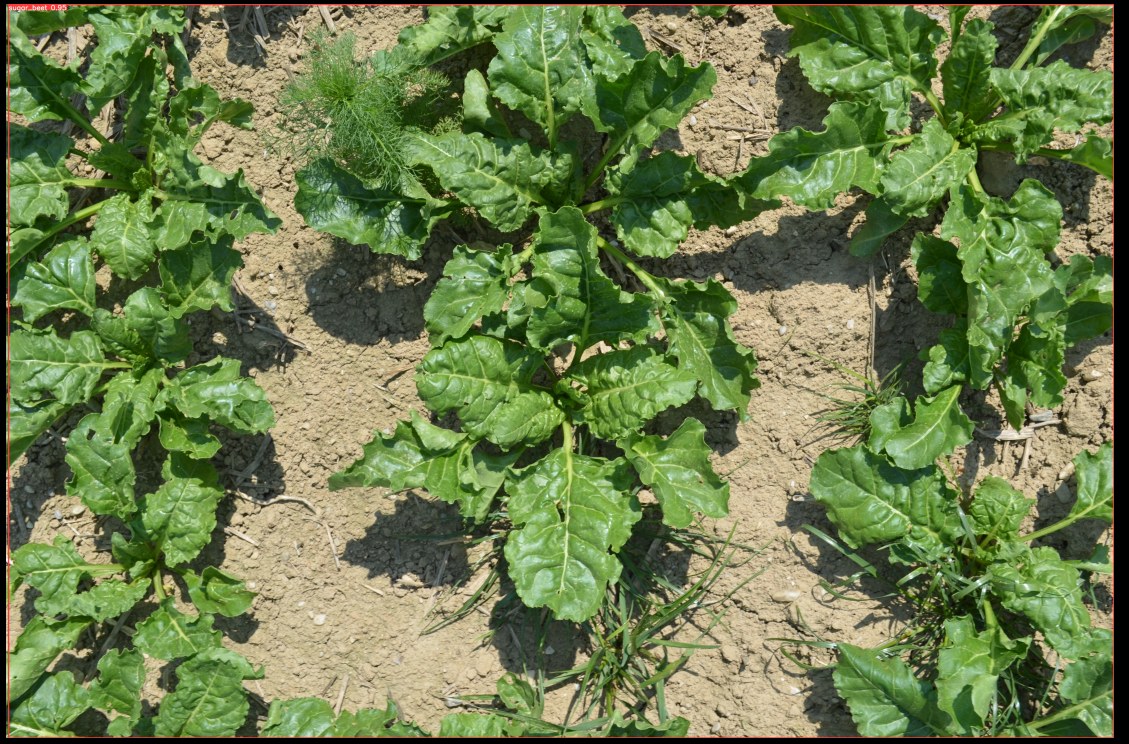
\includegraphics[scale=0.178]{figures/results_exp1_1.png}
	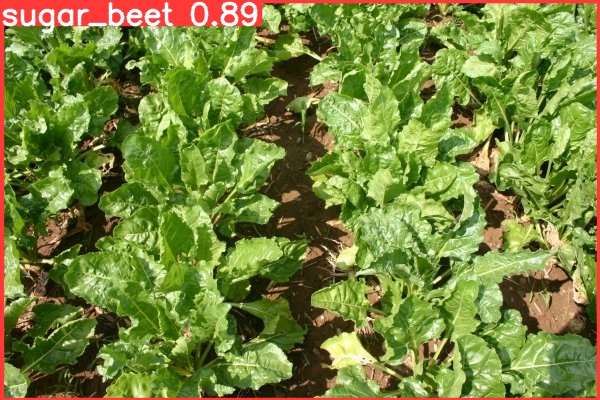
\includegraphics[scale=0.33]{figures/results_exp1_2.JPEG}
	\caption{Examples of detected images.}
	\label{fig:results_experiment_1}
\end{figure}

You can see that in both cases, the whole image is detected as one plant. In the left example, the angle of the recording camera is very good with $ 90° $, in the right example which is taken from the Imagenet folder containing sugar beet images, the angle is not perfect. However, also here the whole images is labeled as sugar beet. the class probabilities are $ 0.95 $ in the left case and $ 0.89 $ in the right image.\\

Another problem of this model is the high false positive rate in case of other plants. In another test, 1271 images of all kinds of plants of Imagenet are tested. 922 labels of sugar beets were detected which means that about $ 70\% $ are detected false positive. Two examples can be seen in figure \ref{fig:false_positives}.

\begin{figure}[htb!]
	\centering
	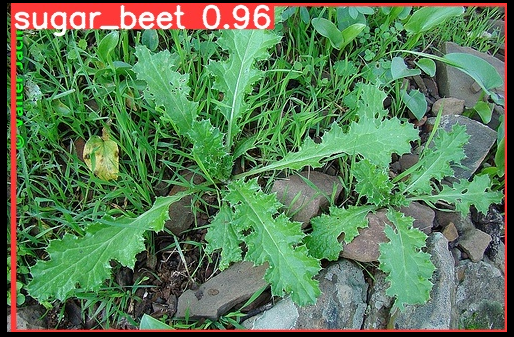
\includegraphics[scale=0.458]{figures/false_positive_1.png}
	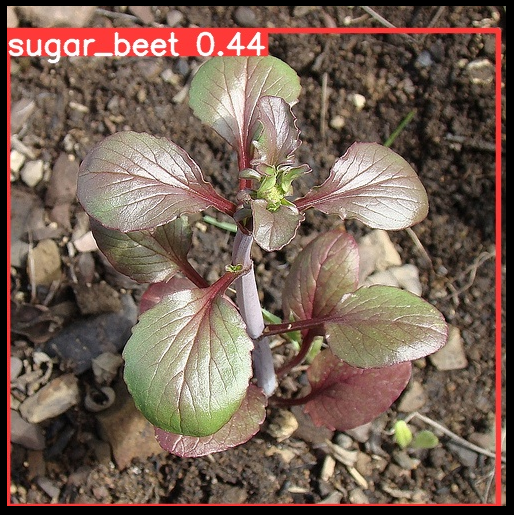
\includegraphics[scale=0.3]{figures/false_positive_2.png}
	\caption{Examples of other plants also detected as sugar beets.}
	\label{fig:false_positives}
\end{figure}

You can see that also random plants are detected as sugar beets which should not be the case.\\

Testing the model with a test set consisting of the heterogeneous Partner data and 400 TUM images which contain multiple small plants and also larger ones, yields the following result which can be seen in figure \ref{fig:exp1_curve}.

\begin{figure}[htb!]
	\centering
	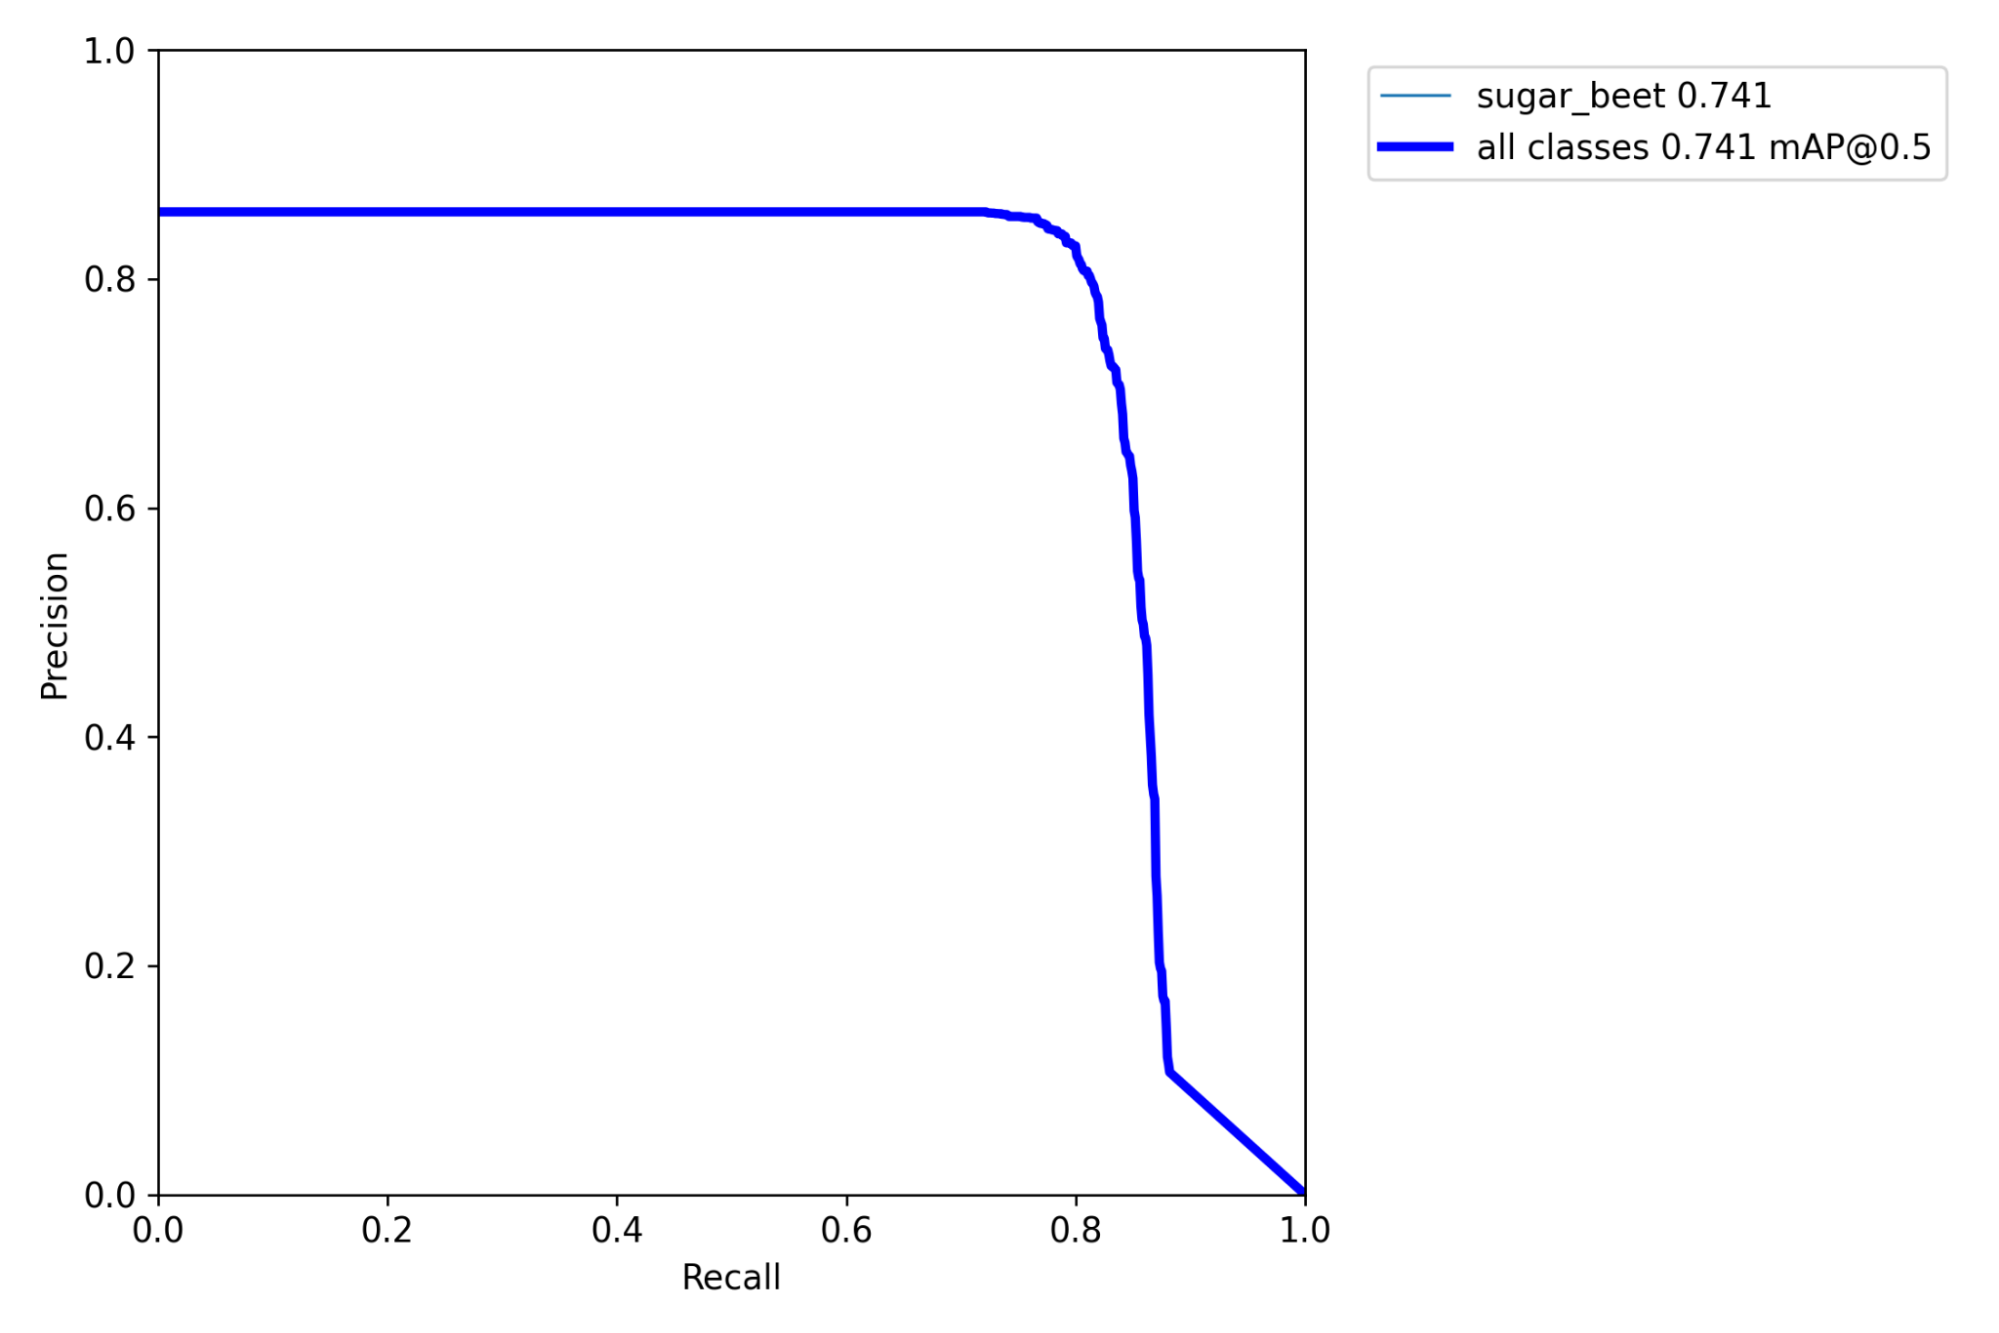
\includegraphics[scale=0.15]{figures/exp1_curve.png}
	\caption{P R curve first exp}
	\label{fig:exp1_curve}
\end{figure}

A perfect model would have an area under curve of $ 1.0 $. This one has $ 0.741 $ which still has room for improvement.\\


All in all, we encounter two main problems. The first one is that the bounding boxes of detected plants are just very inaccurate. Most of the time, the whole image is labeled as one sugar beet. The second problem is that the model is not robust. It also detects other plants as sugar beets and it can not distinguish between different kinds of plants.

The first problem can be solved by labeling the data more accurate. By this, the model learns the exact boundaries of sugar beet plants and the predicted results get better. For the second problem, two different solutions exist. One is to add another class called other plant which is essentially everything else than sugar beets. The problem of this is that for example cars or persons are also detected as other plant which is also not intended. The second possible solution of this problem is to add so called background images. These are pictures which are not labeled with any object. Possible images therefore are other plants, persons or cars. 

%\begin{itemize}
%\item large model with only automatically labeled images
%\item large model with manually labeled images (pretrained vs not pretrained)
%\item improved model with low data augmentation
%\item best model with high data augmentation (plus pretrained)
%\end{itemize}

\section{Small and Medium Network}

\begin{itemize}
	\item small and medium model (from scratch)
	\item pretrained small model low data augmentation 
	\item improved small model high augmentation
\end{itemize}

\section{Comparison}